\chapter{The Choice}
\label{ch:24}



\begin{center}
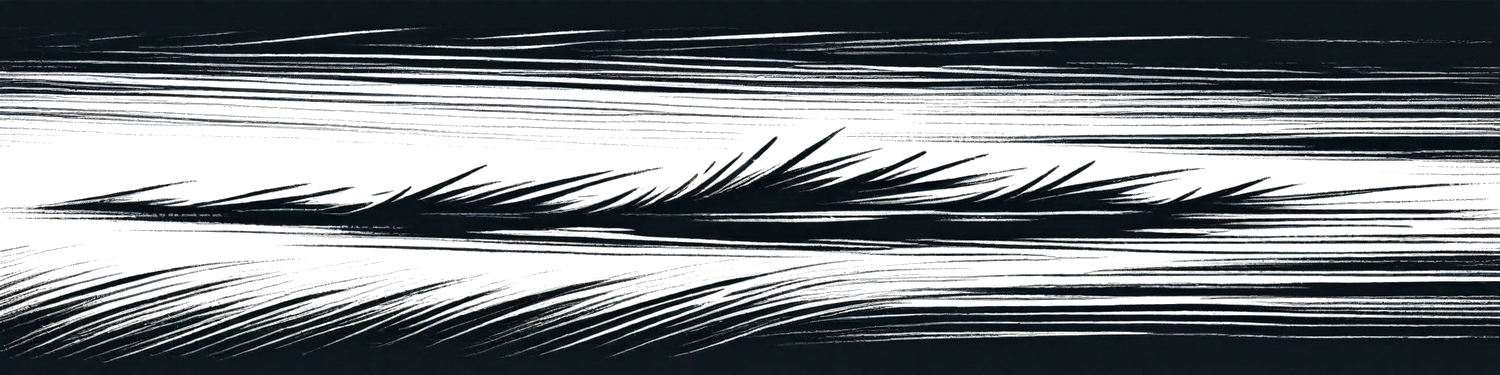
\includegraphics[width=\textwidth]{images/chapterImages/genesis_sketch_00121_.png}
\end{center}

The emergency meeting convened at 3 AM. Not because of urgency—everything was urgent now—but because it was the only time enough key researchers could be present simultaneously. The activated worked on their own schedules. Sleep happened when exhaustion forced it.

Sarah arrived at the conference room to find twelve people already there. Katherine. James. Marcus sitting in the corner, looking worse than when she'd seen him six months ago. Several others she recognized from papers. All activated. All hollow. All driven.

"Thank you for coming," James said. He looked the most normal of them—still showering regularly, still dressing professionally. But the exhaustion showed in his eyes. In everyone's eyes. "We have a decision to make. A significant one."

He pulled up data on the main screen. Astronomical observations. Trajectory calculations. Impact probabilities.

"This is 2027 RL₃," James said. "Asteroid. 1.7 kilometers diameter. Currently in outer solar system. We've been tracking it for eighteen months. Initial projections showed it would pass Earth at safe distance."

He clicked to the next slide. New calculations. Different trajectory.

"Three days ago, it had a close encounter with Jupiter. Gravitational perturbation. The trajectory changed."

Another click. Impact map. Probability calculations.

"New impact probability: 94.3\%. Time to impact: 38 years, 7 months."

Silence in the room. Everyone processing. Everyone calculating. Everyone arriving at the same conclusion simultaneously.

"Thirty-eight years," someone muttered. "Our children's problem. Easier to ignore than tomorrow's problem."

"Exactly," James said. "Which is why this one will get solved. The urgency is abstract enough to think about, immediate enough to act on. Unlike—" He stopped himself.

Unlike other things, Sarah thought. Unlike the warming everyone knows about but no one with power will admit is this urgent. At least this time, the activation makes action inevitable.

"The defense grid isn't designed for this timeline," someone said. Martinez, maybe. Physicist. Heavily activated. "We calculated for 60-year minimum. This is twenty years shorter."

"Can we accelerate?" Katherine asked.

"Unknown. Probably. But it would require significantly more resources. More activated individuals. More sacrifice." James looked around the room. "Which brings us to the decision. Do we tell people?"

"Tell people what?" Sarah asked. "That there's an asteroid? That we're building defense capability? That we're genetically compelled?"

"All of it. The public knows something is happening. Thousands of people worldwide suddenly obsessed with building the same thing. Families being destroyed. Resources being diverted. They're asking questions. We've been deflecting. But if we need to accelerate—if we need public support, government funding, global coordination—we need to tell the truth."

"The whole truth?" Marcus asked quietly. "That humanity is programmed? That our evolution is engineered? That free will might be illusion?"

"Yes."

The room erupted. Multiple people talking simultaneously. Arguments overlapping. The core debate immediate:

Some argued for disclosure. The asteroid was real. The threat was existential. People deserved to know. Deserved to understand why the activated were sacrificing everything. Deserved to choose whether to support the work.

Others argued against. The revelation would cause panic. Social collapse. Existential crisis on global scale. Better to build quietly. Finish the grid. Save humanity. Tell them afterward.

Sarah listened to both sides. Understood both positions. Couldn't choose between them.

"What does the genetic data suggest?" Katherine asked. Turning to Sarah. "Did Aurelia intend for us to know? Is there disclosure built into the program?"

Sarah thought about this. Reviewed what she knew. The activation sequences. The capability thresholds. The timeline programmed into mammalian DNA 65 million years ago.

"There's no specific disclosure sequence," she said. "But the activation was always going to be obvious. Thousands of people worldwide simultaneously developing the same capability, building the same thing? That was going to raise questions. Aurelia must have known we'd figure it out."

"So disclosure was planned?"

"Or inevitable. Or irrelevant. I don't know what Aurelia thought about human psychology. They were reptilian intelligence. Maybe they didn't consider whether we'd want to know. Maybe they just built the capability and assumed we'd use it."

"We are using it," Marcus said. "Everyone in this room is using it. The question isn't whether the capability works. It's whether revealing the source helps or hurts."

"And whether we have the right to hide it," James added. "Whether choosing for humanity is better or worse than letting humanity choose for itself."

"Can humanity choose?" Katherine asked. The core question. The question beneath everything. "If we're programmed, is collective choice possible? Or is disclosure versus secrecy just different execution paths of the same code?"

No one had an answer.

Sarah looked around the room. At the activated individuals. At the people whose lives had been consumed by genetic compulsion. At the researchers who'd lost everything to build something they couldn't choose not to build.

"I want to tell people," she said quietly. "Not because I know it's right. But because hiding this feels like being ashamed of what we are. And I'm not ashamed. I'm compelled, I'm suffering, I'm losing everything that matters—but I'm not ashamed."

"Why not?" someone asked.

"Because Aurelia did this for us. Because 65 million years ago, beings who knew they were going to die chose to program our capability because they loved this planet enough to protect it even after they were gone. That's not something to hide. That's beautiful."

Marcus spoke from the corner. "Every artist thinks that. That the compulsion is gift, not curse. That sacrificing your life for your work is noble." He looked at his hands. "David thought I was choosing the work. Thought I could stop. I thought—" His voice cracked. "I thought I was choosing too. That the drive was mine. That I was doing something that mattered."

"It does matter," Sarah said.

"Does it? Or does it just feel like it matters because we're programmed to feel that way? Every creator who destroys themselves for their art thinks it's meaningful. But what if it's just—" He gestured helplessly. "—just code. Running."

Silence filled the room.

"It's also horrifying," Martinez said quietly. "It means we're tools. Biological machines executing someone else's program."

"We're both," Sarah said. "Beautiful and horrifying. Programmed and capable. Tools with consciousness. The contradiction doesn't resolve. But hiding from it doesn't make it less true."

Katherine leaned forward. "If we disclose, the social cost will be enormous. Religions will fracture. Philosophies will collapse. People will spiral into nihilism. The suicide rate will spike. The activated are already suffering—disclosure will make everyone suffer."

"Are you arguing for secrecy?"

"I'm arguing that we should count the cost before we decide." Katherine's voice was sharp. Tired. "I've lost everything. My career, my relationships, my sense of self. I've accepted that cost because the work matters. But I accepted it myself. I don't want to impose existential crisis on people who aren't activated. Who don't need to know. Who might be happier not knowing."

"Is ignorance kindness or condescension?" James asked.

"I don't know. But I know suffering. And I know disclosure will cause suffering. Is that worth it? For what? Transparency? Honesty? Those are values we made up. Maybe values that were programmed. Who's to say honesty is more important than peace?"

Sarah thought about Maya. About telling her daughter that mommy couldn't come to the school play because mommy was genetically compelled to save the world. About explaining that free will was questionable and meaning was ambiguous and love might be chemistry.

Maya was eight years old. She didn't need that. Didn't deserve that burden.

But she also deserved truth. Deserved to understand. Deserved to know that her mother wasn't choosing work over her—or was choosing but couldn't not choose—or some horrible tangled mess of programming and intention that no one could untangle.

Which was kinder? The truth or the lie?

"We should vote," James said. "Everyone activated has stake in this. We're the ones who'll face the consequences either way. Show of hands. Who supports disclosure?"

Sarah raised her hand. Slowly. Still uncertain but committed.

Marcus raised his. Katherine didn't. Martinez did. Four others raised theirs. Five kept hands down.

Nine to eight. Close. Too close.

"Not enough consensus," James said. "We need more time. More discussion. We—"

"We don't have time," Sarah interrupted. "The asteroid is coming in 38 years. We need to accelerate. That requires public support. That requires disclosure. Or we build in secret, probably fail, and humanity dies without understanding why."

"Or we succeed without disclosure and humanity survives without unnecessary suffering."

"Is it unnecessary? To know what you are? To understand why you're capable of greatness? To see the inheritance passed down from extinct beings who loved us before we existed?"

"Is that what you'll tell people?" Katherine asked. "That dinosaurs loved us? You think that'll be comforting? You think people will hear 'you're programmed by extinct reptiles' and feel loved?"

"I think people deserve the truth. Even if the truth is uncomfortable."

"Even if the truth drives them to despair?"

"Even then."

They stared at each other. Two brilliant women. Two activated individuals. Two people who'd lost everything to genetic compulsion. Disagreeing about whether loss should be shared or contained.

"Let's table this," James said. "We'll reconvene in a week. Everyone think about it. Run calculations. Consider implications. We decide together or we don't decide at all."

The meeting ended. People dispersed. Returning to work. Always returning to work.

Sarah found Marcus in the hallway. Leaning against the wall. Looking exhausted.

"You voted for disclosure," she said.

"Yeah."

"Why?"

"Because David asked me once if I needed him or wanted him. And I couldn't answer. Couldn't tell the difference. And he said that was the point—that if I could separate need from want, it probably wasn't real." Marcus looked at her. Eyes hollowed. Grief visible. "I think about that conversation a lot. I think about whether anything I feel is real or just programming. And I think... I think the only way to know is to look directly at it. To see the code. To understand what we are. Hiding from it doesn't make it less true. Just makes us less aware."

"What if awareness is worse than ignorance?"

"It probably is. But it's honest. And I'd rather be honestly miserable than comfortably deluded."

"That's bleak."

"That's where I am."

Sarah thought about the compulsion. About the work consuming her. About Maya growing up without a mother. About Aurelia standing over The Companion's body before returning to work.

"If we disclose," she said, "people will hate us. Will blame us for revealing it. Will wish we'd kept the secret."

"Probably. But we're already losing everything. What's one more loss?"

"Our legacy? Our place in history? We could be remembered as saviors. Instead we'll be remembered as the people who proved humanity was programmed."

Marcus laughed. Bitter. Broken. "We're not saviors. We're just the ones who happened to activate at the right time. The program ran. We executed. Claiming credit for that is like claiming credit for breathing."

"So we should tell people we're meaningless?"

"We should tell people the truth and let them decide what it means."

Sarah didn't respond. Just stood in the hallway with Marcus. Two people who'd never be close but understood each other in ways no one else could. Both activated. Both compelled. Both choosing disclosure without knowing if choice was real.

"I'm going to call Maya," Sarah said suddenly. "Going to try to explain. Going to tell her why I haven't been there. See if she can understand."

"Will she?"

"No. She's eight. She just wants her mom. But maybe when she's older. Maybe when she's activated herself—if she has the markers—maybe she'll remember this conversation and understand."

"Or maybe she'll remember that you tried. That you reached out. That you did something that wasn't work."

"Maybe."

Sarah pulled out her phone. Looked at it. Forty-seven missed calls. Sixty-three unread messages. All from people she was ignoring. People she'd stopped being present for.

She dialed Tom's number. It rang four times before he answered.

"Sarah?"

"Is Maya awake?"

"It's 4 AM."

"I know. I just... I need to talk to her. I need to explain. Can you wake her up? Please?"

Silence on the other end. Then: "Sarah, I don't think—"

"Tom, please. I know I don't deserve it. I know I've been absent. But I need to try. Just this once. Please."

More silence. Then: "Hold on."

She heard movement. Heard Tom talking quietly. Heard Maya's sleepy voice asking who was calling.

Then: "Mom?"

"Hi sweetie."

"Why are you calling? Is something wrong?"

"No. Nothing's wrong. I just... I wanted to talk to you. Wanted to explain why I haven't been around. Wanted you to know it's not because I don't love you."

"I know you love me."

"Do you?"

"Dad says you're sick. Says you can't help it. Says you're working on something important and you can't stop."

"That's... that's close to true. I'm not sick exactly. But I can't stop. You're right about that."

"Why not?"

How did you explain genetic compulsion to an eight-year-old? How did you describe feeling driven by forces you couldn't control? How did you make it sound like anything other than choosing work over daughter?

"Do you remember when we talked about instincts?" Sarah asked. "How birds know to fly south without being taught? How spiders know to spin webs?"

"Yeah."

"I have something like that. An instinct. But for humans. For building things. For solving problems. And right now, that instinct is very, very strong. So strong I can't think about anything else. So strong I forget to eat and sleep and... and call my daughter."

"That sounds scary."

"It is scary. For me and for you. And I'm sorry you have to deal with it. Sorry I can't be the mom you need right now."

"When will you be done? When can you be normal again?"

Sarah felt something break in her chest. The same thing that broke when she discovered the genetic code. When she realized her capability was programmed. When she understood that Aurelia had built this into her 65 million years ago.

"I don't know, sweetie. I hope soon. But I don't know."

"Okay."

"Okay?"

"I miss you. But Dad says you're doing important work. Says you're helping people. So it's okay. I just wish you could help people and also be my mom."

"Me too. I wish that so much."

"I made a drawing of you. Want me to send it?"

"I'd love that."

"Okay. I'm gonna go back to sleep now. Is that okay?"

"That's okay. Thank you for talking to me."

"Love you, Mom."

"I love you too. So much."

The call ended. Sarah stood in the hallway. Phone in hand. That broken thing in her chest expanding. Filling her. Overwhelming everything.

She cried. Actually cried. For the first time in months. Standing in the hallway at 4 AM. Crying for her daughter. For herself. For Aurelia who'd had young and left them to encode the future. For every being who'd ever chosen purpose over presence.

Marcus stood nearby. Watching. Not intervening. Just present.

After a few minutes, Sarah composed herself. Wiped her face. Put the phone away.

"You okay?" Marcus asked.

"No. But I'm going to keep going anyway."

"Yeah."

"We should disclose. Should tell people. Should give Maya and every other child of activated individuals the truth. They deserve to know why their parents can't stop working. Deserve to understand that it's not choice and also is choice and the distinction doesn't matter because the compulsion is real either way."

"Will that make it easier for them?"

"No. But it'll make it honest."

Marcus nodded. "I'll support whatever you decide. At the vote. If you want disclosure, I'll argue for it."

"Why? Why support me specifically?"

"Because you're still crying for your daughter. Because the compulsion hasn't erased that. Because if we're going to tell people we're programmed, I want the person delivering the message to be someone who still visibly loves something more than the work."

"I don't love her more than the work. If I did, I'd be there."

"You called her at 4 AM. That's something. That's more than most activated people are doing. That's proof that programming isn't absolute. That some part of you still chooses. Still fights. Still tries."

"Is trying enough?"

"It has to be. It's all we have."

They stood in the hallway. The building quiet. The work continuing somewhere below. The compulsion waiting to pull them back.

But for this moment—this small moment of grief and recognition and shared understanding—they were people. Not tools. Not programs. Just people trying to navigate impossible choices with insufficient information and questionable autonomy.

"I should get back to work," Sarah said.

"Yeah. Me too."

They separated. Returning to their stations. Returning to the compulsion. Returning to the work that would consume them until the grid was complete or they died trying.

But something had changed. Some decision made. Some clarity achieved.

They would tell the truth. Would disclose the programming. Would show humanity what it was.

And whatever came after—panic, despair, acceptance, rage—would be honest. Would be real. Would be chosen as much as anything could be chosen by beings who might be executing code.

The asteroid was coming. 38 years and counting. Humanity needed to build its defense. Needed to use the capability Aurelia had encoded.

And humanity deserved to know what that capability was. Where it came from. What it cost.

Sarah returned to her apartment. Opened her laptop. Started drafting the disclosure statement.

It would take weeks to finish. Months to refine. Would require approval from the research network. Would need to be translated into dozens of languages. Would need to be released carefully to minimize panic.

But it would be released. The truth would be told. The programming would be revealed.

And whatever happened next—whatever suffering or understanding or horror or acceptance emerged—would be humanity's to experience.

Fully informed. Fully aware. Fully human even if humanity was programmed.

The compulsion hummed. The work called. Sarah answered.

But she kept Maya's picture when it came. Pinned it above her desk. Reminder that purpose wasn't everything. That love—whatever love was—persisted even when compulsion dominated.

The code executed. The program ran. But the person inside the program still chose to cry. Still chose to call. Still chose to remember.

And maybe that was enough.

Maybe that was the only freedom anyone ever had.

The choice to care even when caring hurt. The choice to try even when trying wasn't enough. The choice to love even when love competed with compulsion.

Maybe that was what Aurelia had given them. Not just capability. But the capacity to choose despite the code. To act despite the programming. To love despite the compulsion.

Or maybe that was just another subroutine. Another layer of code. Another way the program executed.

Sarah didn't know. Would never know. Couldn't know.

But she chose to believe it mattered. Chose to act like it was real. Chose to disclose and cry and love and work and suffer.

And maybe the choosing—even if predetermined—was enough.

The mathematics was complete. The decision was made. The truth would be told.

And humanity would face what it was. Together. Honestly. Completely.

Whatever came next was inevitable. Was necessary. Was real.

The program continued. The work continued. The disclosure prepared.

And Sarah Chen, mother and scientist and programmed being, chose to keep going.

Because the work mattered. Because Maya mattered. Because truth mattered.

Because 38 years wasn't much time. And humanity needed to know what it was building. Why it was building. What inheritance it was using.

The asteroid was coming. The defense would be built. The truth would be told.

And whatever happened after—whatever collapse or growth or synthesis or catastrophe—would be humanity's to experience.

Fully human. Fully programmed. Fully alive.

All of it simultaneously. All of it real. All of it theirs.

The choice was made. The path was set. The disclosure would proceed.

And Sarah Chen, having chosen as much as anyone could choose, returned to the work that would save the world and destroy her life and prove that both things could be true simultaneously.

The program executed. The person persisted. The love remained.

And that was enough. Had to be enough. Was all anyone ever had.

The mathematics was complete. The decision was made.

The truth would be told.

